\chapter{Algorismes de cadenes}

Aquest capítol tracta sobre algorismes eficients per al processament
de cadenes. Molts problemes de cadenes es poden resoldre fàcilment en
temps $O(n^2)$, però el repte és trobar algorismes que funcionin en
temps $O(n)$ o $O(n \log n)$.

\index{cerca de patró}

Per exemple, un problema fonamental de processament de cadenes és el
problema de cercar de patró (\key{pattern matching}): donada una
cadena de longitud $n$ i un patró de longitud $m$, la nostra tasca és
trobar les ocurrències del patró a la cadena. Per exemple, el patró
\texttt{ABC} apareix dues vegades a la cadena \texttt{ABABCBABC}.

El problema de cerca de patrons es pot resoldre fàcilment en temps
$O(nm)$ mitjançant un algorisme de força bruta que prova totes les
posicions on es pot produir el patró a la cadena. En aquest capítol
veurem que hi ha algorismes més eficients que només requereixen temps
$O(n+m)$.

\index{cadena}

\section{Terminologia de cadenes}

\index{alfabet}

Al llarg del capítol, assumim que la indexació en base zero s'utilitza
a les cadenes. Així, una cadena \texttt{s} de longitud $n$ consta de
caràcters $\texttt{s}[0],\texttt{s}[1],\ldots,\texttt{s}[n-1]$ . El
conjunt de caràcters que poden aparèixer a les cadenes s'anomena
\key{alfabet}. Per exemple, l'alfabet
$\{\texttt{A},\texttt{B},\ldots,\texttt{Z}\}$ consta de les majúscules
de l'anglès.

\index{subcadena}

Una \key{subcadena} és una seqüència de caràcters consecutius en una
cadena. Utilitzem la notació $\texttt{s}[a \ldots b]$ per referir-nos
a una subcadena de \texttt{s} que comença a la posició $a$ i acaba a
la posició $b$. Una cadena de longitud $n$ té $n(n+1)/2$
subcadenes. Per exemple, les subcadenes de \texttt{ABCD} són
\texttt{A}, \texttt{B}, \texttt{C}, \texttt{D}, \texttt{AB},
\texttt{BC}, \texttt {CD}, \texttt{ABC}, \texttt{BCD} i \texttt{ABCD}.

\index{subseqüència}

Una \key{subseqüència} és una seqüència de caràcters (no
necessàriament consecutius) en una cadena en el seu ordre
original. Una cadena de longitud $n$ té $2^n-1$ subseqüències. Per
exemple, les subseqüències de \texttt{ABCD} són \texttt{A},
\texttt{B}, \texttt{C}, \texttt{D}, \texttt{AB}, \texttt{AC}, \texttt
       {AD}, \texttt{BC}, \texttt{BD}, \texttt{CD}, \texttt{ABC},
       \texttt{ABD}, \texttt{ACD}, \texttt{BCD} i \texttt{ABCD}.

\index{prefix} \index{sufix}

Un \key{prefix} és una subcadena que comença al principi d'una cadena,
i un \key{sufix} és una subcadena que acaba al final d'una
cadena. Per exemple, els prefixos de \texttt{ABCD} són \texttt{A},
\texttt{AB}, \texttt{ABC} i \texttt{ABCD}, i els sufixos de
\texttt{ABCD} són \texttt{D}, \texttt{CD}, \texttt{BCD} i
\texttt{ABCD}.

\index{rotació}

Es pot generar una \key{rotació} movent els caràcters d'una cadena un
per un del principi al final (o viceversa). Per exemple, les rotacions
de \texttt{ABCD} són \texttt{ABCD}, \texttt{BCDA}, \texttt{CDAB} i
\texttt{DABC}.

\index{període}

Un \key{període} és un prefix d'una cadena de manera que la cadena es
pot construir repetint el període. L'última repetició pot ser parcial i
contenir només un prefix del període. Per exemple, el període més curt de
\texttt{ABCABCA} és \texttt{ABC}.

\index{vora}

Una \key{vora} (\emph{border}) és una subcadena que és alhora un
prefix i un sufix d'una cadena. Per exemple, les vores de
\texttt{ABACABA} són \texttt{A}, \texttt{ABA} i \texttt{ABACABA}.

\index{ordre lexicogràfic}

Les cadenes es comparen utilitzant l'\key{ordre lexicogràfic} (que
correspon a l'ordre alfabètic). Diem que $x<y$ si $x \neq y$ i
$x$ és un prefix de $y$, o si hi ha una posició $k$ tal que $x[i]=y[i]$
quan $i<k$ i $x[k]<y[k]$.

\section{Tipus Trie}

\index{trie}

Un \key{trie}, o arbre de prefixes, és un arbre arrelat que representa
un conjunt de cadenes. Cada cadena del conjunt s'emmagatzema com una
cadena de caràcters que comença a l'arrel. Si dues cadenes tenen un
prefix comú, també tenen una cadena comuna a l'arbre.

Per exemple, considereu el trie següent:


\begin{center}
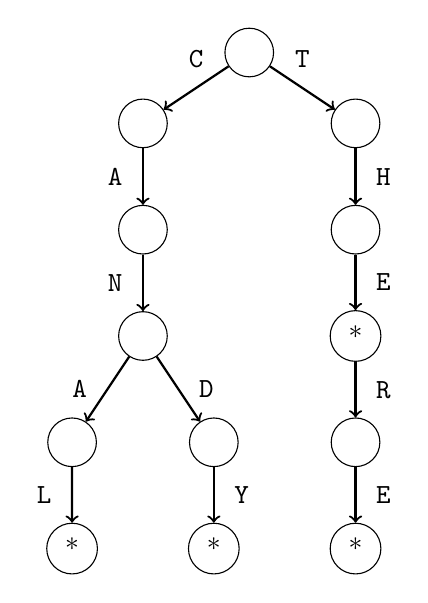
\begin{tikzpicture}[scale=0.9]
\node[draw, circle] (1) at (0,20) {$\phantom{1}$};
\node[draw, circle] (2) at (-1.5,19) {$\phantom{1}$};
\node[draw, circle] (3) at (1.5,19) {$\phantom{1}$};
\node[draw, circle] (4) at (-1.5,17.5) {$\phantom{1}$};
\node[draw, circle] (5) at (-1.5,16) {$\phantom{1}$};
\node[draw, circle] (6) at (-2.5,14.5) {$\phantom{1}$};
\node[draw, circle] (7) at (-0.5,14.5) {$\phantom{1}$};
\node[draw, circle] (8) at (-2.5,13) {*};
\node[draw, circle] (9) at (-0.5,13) {*};
\node[draw, circle] (10) at (1.5,17.5) {$\phantom{1}$};
\node[draw, circle] (11) at (1.5,16) {*};
\node[draw, circle] (12) at (1.5,14.5) {$\phantom{1}$};
\node[draw, circle] (13) at (1.5,13) {*};

\path[draw,thick,->] (1) -- node[font=\small,label=\texttt{C}] {} (2);
\path[draw,thick,->] (1) -- node[font=\small,label=\texttt{T}] {} (3);
\path[draw,thick,->] (2) -- node[font=\small,label=left:\texttt{A}] {} (4);
\path[draw,thick,->] (4) -- node[font=\small,label=left:\texttt{N}] {} (5);
\path[draw,thick,->] (5) -- node[font=\small,label=left:\texttt{A}] {} (6);
\path[draw,thick,->] (5) -- node[font=\small,label=right:\texttt{D}] {} (7);
\path[draw,thick,->] (6) -- node[font=\small,label=left:\texttt{L}] {}(8);
\path[draw,thick,->] (7) -- node[font=\small,label=right:\texttt{Y}] {} (9);
\path[draw,thick,->] (3) -- node[font=\small,label=right:\texttt{H}] {} (10);
\path[draw,thick,->] (10) -- node[font=\small,label=right:\texttt{E}] {} (11);
\path[draw,thick,->] (11) -- node[font=\small,label=right:\texttt{R}] {} (12);
\path[draw,thick,->] (12) -- node[font=\small,label=right:\texttt{E}] {} (13);
\end{tikzpicture}
\end{center}


Aquest trie correspon al conjunt
$\{\texttt{CANAL},\texttt{CANDY},\texttt{THE},\texttt{THERE}\}$. El
caràcter * en un node significa que una cadena del conjunt acaba al
node. Aquest caràcter és necessari, perquè una cadena pot ser un
prefix d'una altra cadena. Per exemple, a la prova anterior,
\texttt{THE} és un prefix de \texttt{THERE}.

Podem comprovar en temps $O(n)$ si un trie conté una cadena de
longitud $n$, perquè podem seguir la cadena començant al node
arrel. També podem afegir una cadena de longitud $n$ al trie en temps
$O(n)$, seguint primer la cadena i després afegint nous nodes al trie
si cal.

Si representem un conjunt com a trie, podem trobar, donada una cadena,
quin és el prefix més llarg que pertanyi al conjunt. Si afegim
informació addicional als nodes del trie també podem calcular el
nombre de cadenes del conjunt que tenen un prefix donat.

Un trie es pot emmagatzemar en una matriu
\begin{lstlisting}
int trie[N][A];
\end{lstlisting}
on $N$ és el nombre màxim de nodes (la longitud total màxima de les
cadenes del conjunt) i $A$ és la mida de l'alfabet. Els nodes d'un
trie estan numerats $0,1,2,\ldots$ de manera que el número de l'arrel
és 0, i $\texttt{trie}[s][c]$ és el següent node de la cadena quan ens
movem del node $s$ utilitzant el caràcter $c$.

\section{Hashing de cadenes}

\index{hashing} \index{hashing de cadenes}

El \key{hashing de cadenes} és una tècnica que ens permet comprovar de manera
eficient si dues cadenes són iguals\footnote{La tècnica va ser
popularitzada per l'algorisme de cerca de patrons Karp-Rabin
\cite{kar87}.}. La idea del hash de cadenes és comparar els valors
hash de les cadenes en lloc dels seus caràcters individuals.

\subsubsection*{Càlcul dels valors hash}

\index{valor hash} \index{hash polinomial}

Un \key{valor hash} d'una cadena és un nombre que es calcula a
partir dels caràcters de la cadena. Si dues cadenes són iguals, els
seus valors hash també són els mateixos, cosa que permet comparar
cadenes en funció dels seus valors hash.

Una manera habitual d'implementar un hash de cadena és amb el
\key{hashing polinomial}, que significa que el valor hash d'una cadena
\texttt{s} de longitud $n$ és
\[(\texttt{s}[0] A^{n-1} + \texttt{s}[1] A^{n-2} + \cdots + \texttt{s}[n-1] A^0) \bmod B  ,\]
on $s[0],s[1],\ldots,s[n-1]$ són els codis dels
caràcters de \texttt{s}, i $A$ i $B$ són constants pre-determinades.

Per exemple, els codis dels caràcters de \texttt{ALLEY} són:
\begin{center}
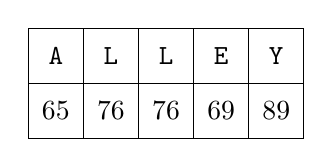
\begin{tikzpicture}[scale=0.7]
\draw (0,0) grid (5,2);

\node at (0.5, 1.5) {\texttt{A}};
\node at (1.5, 1.5) {\texttt{L}};
\node at (2.5, 1.5) {\texttt{L}};
\node at (3.5, 1.5) {\texttt{E}};
\node at (4.5, 1.5) {\texttt{Y}};

\node at (0.5, 0.5) {65};
\node at (1.5, 0.5) {76};
\node at (2.5, 0.5) {76};
\node at (3.5, 0.5) {69};
\node at (4.5, 0.5) {89};

\end{tikzpicture}
\end{center}


Així, si $A=3$ i $B=97$, el valor hash de \texttt{ALLEY} és
\[(65 \cdot 3^4 + 76 \cdot 3^3 + 76 \cdot 3^2 + 69 \cdot 3^1 + 89 \cdot 3^0) \bmod 97 = 52.\]


\subsubsection*{Preprocessament}

Utilitzant el hash polinomial, podem calcular el valor hash de
qualsevol subcadena d'una cadena \texttt{s} en temps $O(1)$ després
d'un preprocessament de temps $O(n)$. La idea és construir un vector
\texttt{h} tal que $\texttt{h}[k]$ contingui el valor hash del prefix
$\texttt{s}[0 \ldots k]$. Els valors del vector es poden calcular
recursivament de la següent manera:
\[
\begin{array}{lcl}
\texttt{h}[0] & = & \texttt{s}[0] \\
\texttt{h}[k] & = & (\texttt{h}[k-1] A + \texttt{s}[k]) \bmod B \\
\end{array}
\]
A més, construïm un vector $\texttt{p}$ on $\texttt{p}[k]=A^k \bmod B$:
\[
\begin{array}{lcl}
\texttt{p}[0] & = & 1 \\
\texttt{p}[k] & = & (\texttt{p}[k-1] A) \bmod B. \\
\end{array}
\]
La construcció d'aquestes matrius requereix temps $O(n)$. Després
d'això, el valor hash de qualsevol subcadena $\texttt{s}[a \ldots b]$
es pot calcular en temps $O(1)$ mitjançant la fórmula
\[(\texttt{h}[b]-\texttt{h}[a-1] \texttt{p}[b-a+1]) \bmod B\]
suposant que $a>0$. Si $a=0$, el valor hash és simplement $\texttt{h}[b]$.

\subsubsection*{Ús dels valors hash}

Podem comparar cadenes de manera eficient mitjançant valors hash. En
lloc de comparar els caràcters individuals de les cadenes, la idea és
comparar els seus valors hash. Si els valors hash són iguals, les
cadenes són \emph{probablement} iguals, i si els valors hash són
diferents, les cadenes són \emph{certament} diferents.

Fent servir hashing, sovint podem fer eficient un algorisme de força
bruta. Per exemple, considerem el problema de cerca de patrons: donada
una cadena $s$ i un patró $p$, trobem les posicions on es produeix $p$
a $s$. Un algorisme de força bruta passa per totes les posicions on es
pot produir $p$ i compara les cadenes caràcter per caràcter. La
complexitat temporal d'aquest algorisme és $O(n^2)$.

Podem fer que l'algorisme de força bruta sigui més eficient utilitzant
hashing, perquè l'algorisme compara subcadenes de cadenes. Utilitzant
el hash, cada comparació només triga $O(1)$ temps, perquè només es
comparen els valors hash de les subcadenes. Això resulta en un
algorisme amb complexitat temporal $O(n)$, que és la millor
complexitat temporal possible per a aquest problema.

Combinant hashing i \emph{cerca binària}, també és possible esbrinar
l'ordre lexicogràfic de dues cadenes en temps logarítmic. Això es pot
fer calculant la longitud del prefix comú de les cadenes mitjançant la
cerca binària. Un cop sabem la longitud del prefix comú, només podem
comprovar el caràcter següent després del prefix, perquè això
determina l'ordre de les cadenes.

\subsubsection*{Col·lisions i paràmetres}

\index{col·lisió}

Un risc evident quan es comparen els valors hash és una
\key{col·lisió}, que vol dir que dues cadenes tenen continguts
diferents però valors hash iguals. En aquest cas, un algorisme que es
basa en els valors hash conclou que les cadenes són iguals, però en
realitat no ho són, i l'algorisme pot donar resultats incorrectes.

Les col·lisions sempre són possibles, perquè el nombre de cadenes
diferents és més gran que el nombre de valors hash
diferents. Tanmateix, la probabilitat d'una col·lisió és petita si es
trien amb cura les constants $A$ i $B$. Una manera habitual és triar
constants aleatòries properes a $10^9$, per exemple de la següent
manera:
\[
\begin{array}{lcl}
A & = & 911382323 \\
B & = & 972663749 \\
\end{array}
\]


Utilitzant aquestes constants, el tipus \texttt{long long} es pot
fer servir quan es calculen els valors hash, perquè els productes $AB$
i $BB$ s'ajustaran a \texttt{long long}. Però n'hi ha prou amb tenir
$10^9$ valors hash diferents?

Considerem tres escenaris en què es pot utilitzar el hash:

\textit{Escenari 1:} Les cadenes $x$ i $y$ es comparen entre si. La
probabilitat d'una col·lisió és $1/B$ assumint que tots els valors
hash són igualment probables.

\textit{Escenari 2:} Es compara una cadena $x$ amb les cadenes
$y_1,y_2,\ldots,y_n$. La probabilitat d'una o més col·lisions és


\[1-(1-\frac{1}{B})^n.\]


\textit{Escenari 3:} Tots els parells de cadenes $x_1,x_2,\ldots,x_n$
es comparen entre si. La probabilitat d'una o més col·lisions és
\[ 1 - \frac{B \cdot (B-1) \cdot (B-2) \cdots (B-n+1)}{B^n}.\]


La taula següent mostra les probabilitats de col·lisió quan $n=10^6$ i
el valor de $B$ varia:


\begin{center}
\begin{tabular}{rrrr}
constant $B$ & scenario 1 & scenario 2 & scenario 3 \\
\hline
$10^3$ & $0.001000$ & $1.000000$ & $1.000000$ \\
$10^6$ & $0.000001$ & $0.632121$ & $1.000000$ \\
$10^9$ & $0.000000$ & $0.001000$ & $1.000000$ \\
$10^{12}$ & $0.000000$ & $0.000000$ & $0.393469$ \\
$10^{15}$ & $0.000000$ & $0.000000$ & $0.000500$ \\
$10^{18}$ & $0.000000$ & $0.000000$ & $0.000001$ \\
\end{tabular}
\end{center}

La taula mostra que a l'escenari 1, la probabilitat d'una col·lisió és
insignificant quan $B \approx 10^9$. En l'escenari 2, és possible una
col·lisió, però la probabilitat és encara bastant petita. Tanmateix, a
l'escenari 3 la situació és molt diferent: gairebé sempre es produirà
una col·lisió quan $B \approx 10^9$.

\index{paradoxa de l'aniversari}

El fenomen de l'escenari 3 es coneix com la \key{paradoxa de
  l'aniversari}: si hi ha $n$ persones a una habitació, la
probabilitat que \emph{algun} parell de persones tingui el mateix
aniversari és gran encara que $n$ sigui bastant petit. En hash, en
conseqüència, quan es comparen tots els valors hash entre si, la
probabilitat que uns dos valors hash siguin iguals és gran.

Podem reduir la probabilitat d'una col·lisió calculant
\emph{múltiples} valors hash amb paràmetres distints, ja que és poc
probable que es produeixi una col·lisió en tots els valors hash al
mateix temps. Per exemple, dos valors hash amb el paràmetre $B \approx
10^9$ corresponen a un valor hash amb el paràmetre $B \approx
10^{18}$, la qual cosa fa que la probabilitat d'una col·lisió sigui
molt petita.

Algunes persones utilitzen constants $B=2^{32}$ i $B=2^{64}$, cosa que
és convenient, perquè les operacions amb enters de 32 i 64 bits es
calculen mòdul $2^{32}$ i $2^{64 }$. Tanmateix, aquesta \emph{no} és
una bona opció, perquè és possible construir entrades que sempre
generin col·lisions quan s'utilitzen constants de la forma $2^x$
\cite{pac13}.

\section{Algorisme Z}

\index{Algorisme Z} \index{Matriu Z}

El \key{Z-vector} \texttt{z} d'una cadena \texttt{s} de longitud $n$
conté per a cada $k=0,1,\ldots,n-1$ la longitud de la subcadena més
llarga de \texttt{s} que comença a la posició $k$ i és un prefix de
\texttt{s}. Així, $\texttt{z}[k]=p$ ens diu que $\texttt{s}[0 \ldots
  p-1]$ és igual a $\texttt{s}[k \ldots k+p-1]$ . Molts problemes de
processament de cadenes es poden resoldre de manera eficient
mitjançant el Z-vector.

Per exemple, el Z-vector de \texttt{ACBACDACBACBACDA} és el següent:


\begin{center}
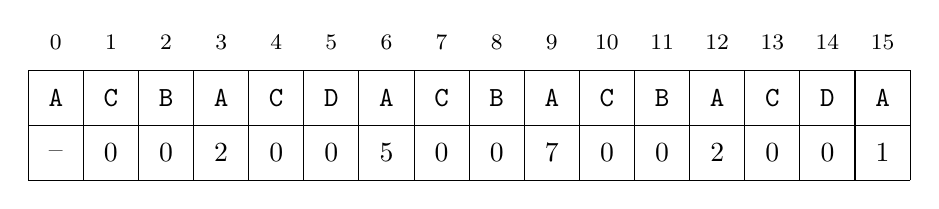
\begin{tikzpicture}[scale=0.7]
\draw (0,0) grid (16,2);

\node at (0.5, 1.5) {\texttt{A}};
\node at (1.5, 1.5) {\texttt{C}};
\node at (2.5, 1.5) {\texttt{B}};
\node at (3.5, 1.5) {\texttt{A}};
\node at (4.5, 1.5) {\texttt{C}};
\node at (5.5, 1.5) {\texttt{D}};
\node at (6.5, 1.5) {\texttt{A}};
\node at (7.5, 1.5) {\texttt{C}};
\node at (8.5, 1.5) {\texttt{B}};
\node at (9.5, 1.5) {\texttt{A}};
\node at (10.5, 1.5) {\texttt{C}};
\node at (11.5, 1.5) {\texttt{B}};
\node at (12.5, 1.5) {\texttt{A}};
\node at (13.5, 1.5) {\texttt{C}};
\node at (14.5, 1.5) {\texttt{D}};
\node at (15.5, 1.5) {\texttt{A}};

\node at (0.5, 0.5) {--};
\node at (1.5, 0.5) {0};
\node at (2.5, 0.5) {0};
\node at (3.5, 0.5) {2};
\node at (4.5, 0.5) {0};
\node at (5.5, 0.5) {0};
\node at (6.5, 0.5) {5};
\node at (7.5, 0.5) {0};
\node at (8.5, 0.5) {0};
\node at (9.5, 0.5) {7};
\node at (10.5, 0.5) {0};
\node at (11.5, 0.5) {0};
\node at (12.5, 0.5) {2};
\node at (13.5, 0.5) {0};
\node at (14.5, 0.5) {0};
\node at (15.5, 0.5) {1};

\footnotesize
\node at (0.5, 2.5) {0};
\node at (1.5, 2.5) {1};
\node at (2.5, 2.5) {2};
\node at (3.5, 2.5) {3};
\node at (4.5, 2.5) {4};
\node at (5.5, 2.5) {5};
\node at (6.5, 2.5) {6};
\node at (7.5, 2.5) {7};
\node at (8.5, 2.5) {8};
\node at (9.5, 2.5) {9};
\node at (10.5, 2.5) {10};
\node at (11.5, 2.5) {11};
\node at (12.5, 2.5) {12};
\node at (13.5, 2.5) {13};
\node at (14.5, 2.5) {14};
\node at (15.5, 2.5) {15};

\end{tikzpicture}
\end{center}


En aquest cas, per exemple, $\texttt{z}[6]=5$, perquè la subcadena
\texttt{ACBAC} de longitud 5 és un prefix de \texttt{s}, però la
subcadena \texttt{ACBACB} de La longitud 6 no és un prefix de
\texttt{s}.

\subsubsection*{Descripció de l'algorisme}

A continuació es descriu un algorisme, anomenat \key{algorisme
  Z}\footnote{L'algorisme Z es va presentar a \cite{gus97} com el
mètode conegut més senzill per a la concordança de patrons en temps
lineal, i la idea original es va atribuir a \ cite{mai84}.}, que
construeix de manera eficient el Z-vector en temps $O(n)$
temps. L'algorisme calcula els valors del Z-vector d'esquerra a
dreta fent servir la informació ja emmagatzemada al Z-vector i
comparant subcadenes caràcter per caràcter.

Per calcular de manera eficient els valors del Z-vector, l'algorisme
manté un rang $[x,y]$ tal que $\texttt{s}[x \ldots y]$ és un prefix
de \texttt{s} i $y$ és tan gran com sigui possible. Com que sabem
que $\texttt{s}[0 \ldots y-x]$ i $\texttt{s}[x \ldots y]$ són iguals,
podem fer servir aquesta informació per calcular els valors Z per a les
posicions $x+1, x+2, \ldots, y$.

A cada posició $k$, primer comprovem el valor de $\texttt{z}[k-x]$. Si
$k+\texttt{z}[k-x]<y$, sabem que
$\texttt{z}[k]=\texttt{z}[k-x]$. Tanmateix, si
$k+\texttt{z}[k-x] \ge y$, aleshores $\texttt{s}[0 \ldots y-k]$ és igual a
$\texttt{s}[k \ldots y]$, i
per determinar la valor de $\texttt{z}[k]$ hem de comparar les
subcadenes caràcter per caràcter. Tot i així, l'algorisme funciona en
temps $O(n)$, perquè comencem a comparar a les posicions $y-k+1$ i
$y+1$.

Per exemple, construïm el Z-vector següent:


\begin{center}
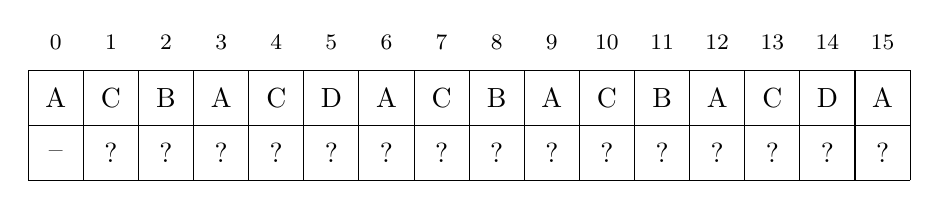
\begin{tikzpicture}[scale=0.7]
\draw (0,0) grid (16,2);

\node at (0.5, 1.5) {A};
\node at (1.5, 1.5) {C};
\node at (2.5, 1.5) {B};
\node at (3.5, 1.5) {A};
\node at (4.5, 1.5) {C};
\node at (5.5, 1.5) {D};
\node at (6.5, 1.5) {A};
\node at (7.5, 1.5) {C};
\node at (8.5, 1.5) {B};
\node at (9.5, 1.5) {A};
\node at (10.5, 1.5) {C};
\node at (11.5, 1.5) {B};
\node at (12.5, 1.5) {A};
\node at (13.5, 1.5) {C};
\node at (14.5, 1.5) {D};
\node at (15.5, 1.5) {A};

\node at (0.5, 0.5) {--};
\node at (1.5, 0.5) {?};
\node at (2.5, 0.5) {?};
\node at (3.5, 0.5) {?};
\node at (4.5, 0.5) {?};
\node at (5.5, 0.5) {?};
\node at (6.5, 0.5) {?};
\node at (7.5, 0.5) {?};
\node at (8.5, 0.5) {?};
\node at (9.5, 0.5) {?};
\node at (10.5, 0.5) {?};
\node at (11.5, 0.5) {?};
\node at (12.5, 0.5) {?};
\node at (13.5, 0.5) {?};
\node at (14.5, 0.5) {?};
\node at (15.5, 0.5) {?};

\footnotesize
\node at (0.5, 2.5) {0};
\node at (1.5, 2.5) {1};
\node at (2.5, 2.5) {2};
\node at (3.5, 2.5) {3};
\node at (4.5, 2.5) {4};
\node at (5.5, 2.5) {5};
\node at (6.5, 2.5) {6};
\node at (7.5, 2.5) {7};
\node at (8.5, 2.5) {8};
\node at (9.5, 2.5) {9};
\node at (10.5, 2.5) {10};
\node at (11.5, 2.5) {11};
\node at (12.5, 2.5) {12};
\node at (13.5, 2.5) {13};
\node at (14.5, 2.5) {14};
\node at (15.5, 2.5) {15};

\end{tikzpicture}
\end{center}


Després de calcular el valor $\texttt{z}[6]=5$, l'interval actual de
$[x,y]$ és $[6,10]$:


\begin{center}
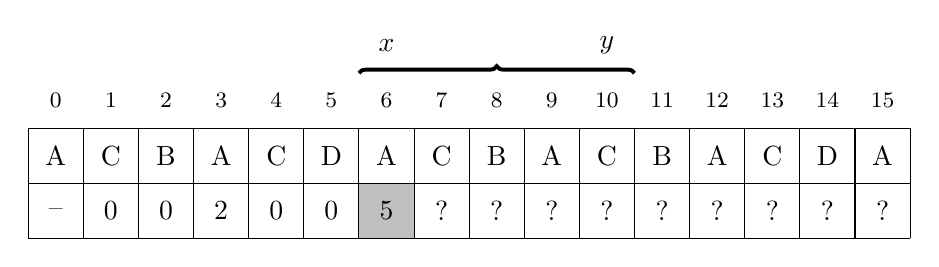
\begin{tikzpicture}[scale=0.7]
\fill[color=lightgray] (6,0) rectangle (7,1);
\draw (0,0) grid (16,2);

\node at (0.5, 1.5) {A};
\node at (1.5, 1.5) {C};
\node at (2.5, 1.5) {B};
\node at (3.5, 1.5) {A};
\node at (4.5, 1.5) {C};
\node at (5.5, 1.5) {D};
\node at (6.5, 1.5) {A};
\node at (7.5, 1.5) {C};
\node at (8.5, 1.5) {B};
\node at (9.5, 1.5) {A};
\node at (10.5, 1.5) {C};
\node at (11.5, 1.5) {B};
\node at (12.5, 1.5) {A};
\node at (13.5, 1.5) {C};
\node at (14.5, 1.5) {D};
\node at (15.5, 1.5) {A};

\node at (0.5, 0.5) {--};
\node at (1.5, 0.5) {0};
\node at (2.5, 0.5) {0};
\node at (3.5, 0.5) {2};
\node at (4.5, 0.5) {0};
\node at (5.5, 0.5) {0};
\node at (6.5, 0.5) {5};
\node at (7.5, 0.5) {?};
\node at (8.5, 0.5) {?};
\node at (9.5, 0.5) {?};
\node at (10.5, 0.5) {?};
\node at (11.5, 0.5) {?};
\node at (12.5, 0.5) {?};
\node at (13.5, 0.5) {?};
\node at (14.5, 0.5) {?};
\node at (15.5, 0.5) {?};

\draw [decoration={brace}, decorate, line width=0.5mm] (6,3.00) -- (11,3.00);

\node at (6.5,3.50) {$x$};
\node at (10.5,3.50) {$y$};


\footnotesize
\node at (0.5, 2.5) {0};
\node at (1.5, 2.5) {1};
\node at (2.5, 2.5) {2};
\node at (3.5, 2.5) {3};
\node at (4.5, 2.5) {4};
\node at (5.5, 2.5) {5};
\node at (6.5, 2.5) {6};
\node at (7.5, 2.5) {7};
\node at (8.5, 2.5) {8};
\node at (9.5, 2.5) {9};
\node at (10.5, 2.5) {10};
\node at (11.5, 2.5) {11};
\node at (12.5, 2.5) {12};
\node at (13.5, 2.5) {13};
\node at (14.5, 2.5) {14};
\node at (15.5, 2.5) {15};

\end{tikzpicture}
\end{center}


Ara podem calcular els valors posterios del Z-vector de manera
eficient, perquè sabem que $\texttt{s}[0 \ldots 4]$ i $\texttt{s}[6
  \ldots 10]$ són iguals. En primer lloc, com que $\texttt{z}[1] =
\texttt{z}[2] = 0$, de seguida sabem que també $\texttt{z}[7] =
\texttt{z}[8] = 0$:


\begin{center}
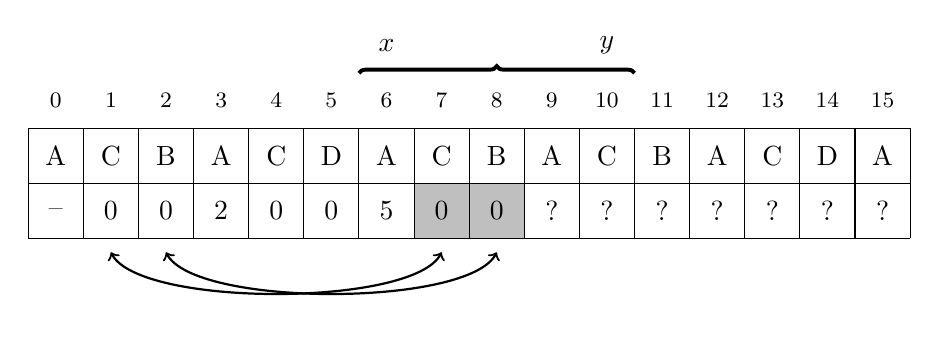
\begin{tikzpicture}[scale=0.7]
\fill[color=lightgray] (7,0) rectangle (9,1);
\draw (0,0) grid (16,2);

\node at (0.5, 1.5) {A};
\node at (1.5, 1.5) {C};
\node at (2.5, 1.5) {B};
\node at (3.5, 1.5) {A};
\node at (4.5, 1.5) {C};
\node at (5.5, 1.5) {D};
\node at (6.5, 1.5) {A};
\node at (7.5, 1.5) {C};
\node at (8.5, 1.5) {B};
\node at (9.5, 1.5) {A};
\node at (10.5, 1.5) {C};
\node at (11.5, 1.5) {B};
\node at (12.5, 1.5) {A};
\node at (13.5, 1.5) {C};
\node at (14.5, 1.5) {D};
\node at (15.5, 1.5) {A};

\node at (0.5, 0.5) {--};
\node at (1.5, 0.5) {0};
\node at (2.5, 0.5) {0};
\node at (3.5, 0.5) {2};
\node at (4.5, 0.5) {0};
\node at (5.5, 0.5) {0};
\node at (6.5, 0.5) {5};
\node at (7.5, 0.5) {0};
\node at (8.5, 0.5) {0};
\node at (9.5, 0.5) {?};
\node at (10.5, 0.5) {?};
\node at (11.5, 0.5) {?};
\node at (12.5, 0.5) {?};
\node at (13.5, 0.5) {?};
\node at (14.5, 0.5) {?};
\node at (15.5, 0.5) {?};


\draw [decoration={brace}, decorate, line width=0.5mm] (6,3.00) -- (11,3.00);

\node at (6.5,3.50) {$x$};
\node at (10.5,3.50) {$y$};


\footnotesize
\node at (0.5, 2.5) {0};
\node at (1.5, 2.5) {1};
\node at (2.5, 2.5) {2};
\node at (3.5, 2.5) {3};
\node at (4.5, 2.5) {4};
\node at (5.5, 2.5) {5};
\node at (6.5, 2.5) {6};
\node at (7.5, 2.5) {7};
\node at (8.5, 2.5) {8};
\node at (9.5, 2.5) {9};
\node at (10.5, 2.5) {10};
\node at (11.5, 2.5) {11};
\node at (12.5, 2.5) {12};
\node at (13.5, 2.5) {13};
\node at (14.5, 2.5) {14};
\node at (15.5, 2.5) {15};


\draw[thick,<->] (7.5,-0.25) .. controls (7,-1.25) and (2,-1.25) .. (1.5,-0.25);
\draw[thick,<->] (8.5,-0.25) .. controls (8,-1.25) and (3,-1.25) .. (2.5,-0.25);
\end{tikzpicture}
\end{center}


Aleshores, com que $\texttt{z}[3]=2$, sabem que $\texttt{z}[9] \ge 2$:


\begin{center}
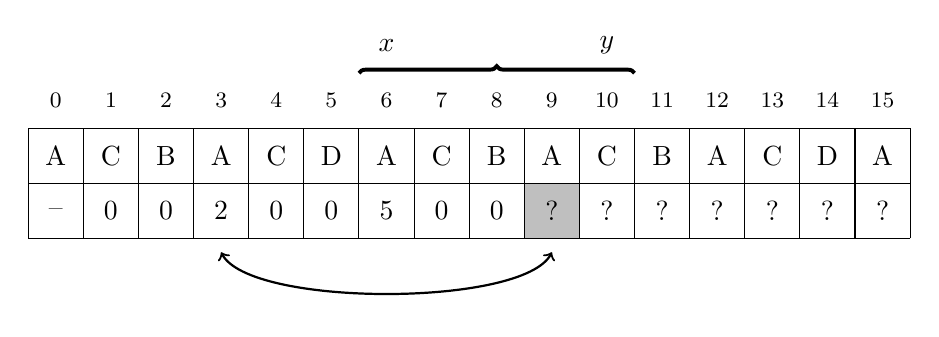
\begin{tikzpicture}[scale=0.7]
\fill[color=lightgray] (9,0) rectangle (10,1);
\draw (0,0) grid (16,2);

\node at (0.5, 1.5) {A};
\node at (1.5, 1.5) {C};
\node at (2.5, 1.5) {B};
\node at (3.5, 1.5) {A};
\node at (4.5, 1.5) {C};
\node at (5.5, 1.5) {D};
\node at (6.5, 1.5) {A};
\node at (7.5, 1.5) {C};
\node at (8.5, 1.5) {B};
\node at (9.5, 1.5) {A};
\node at (10.5, 1.5) {C};
\node at (11.5, 1.5) {B};
\node at (12.5, 1.5) {A};
\node at (13.5, 1.5) {C};
\node at (14.5, 1.5) {D};
\node at (15.5, 1.5) {A};

\node at (0.5, 0.5) {--};
\node at (1.5, 0.5) {0};
\node at (2.5, 0.5) {0};
\node at (3.5, 0.5) {2};
\node at (4.5, 0.5) {0};
\node at (5.5, 0.5) {0};
\node at (6.5, 0.5) {5};
\node at (7.5, 0.5) {0};
\node at (8.5, 0.5) {0};
\node at (9.5, 0.5) {?};
\node at (10.5, 0.5) {?};
\node at (11.5, 0.5) {?};
\node at (12.5, 0.5) {?};
\node at (13.5, 0.5) {?};
\node at (14.5, 0.5) {?};
\node at (15.5, 0.5) {?};

\draw [decoration={brace}, decorate, line width=0.5mm] (6,3.00) -- (11,3.00);

\node at (6.5,3.50) {$x$};
\node at (10.5,3.50) {$y$};


\footnotesize
\node at (0.5, 2.5) {0};
\node at (1.5, 2.5) {1};
\node at (2.5, 2.5) {2};
\node at (3.5, 2.5) {3};
\node at (4.5, 2.5) {4};
\node at (5.5, 2.5) {5};
\node at (6.5, 2.5) {6};
\node at (7.5, 2.5) {7};
\node at (8.5, 2.5) {8};
\node at (9.5, 2.5) {9};
\node at (10.5, 2.5) {10};
\node at (11.5, 2.5) {11};
\node at (12.5, 2.5) {12};
\node at (13.5, 2.5) {13};
\node at (14.5, 2.5) {14};
\node at (15.5, 2.5) {15};

\draw[thick,<->] (9.5,-0.25) .. controls (9,-1.25) and (4,-1.25) .. (3.5,-0.25);
\end{tikzpicture}
\end{center}


Tanmateix, no tenim informació sobre la cadena després de la posició
10, de manera que hem de comparar les subcadenes caràcter per
caràcter:


\begin{center}
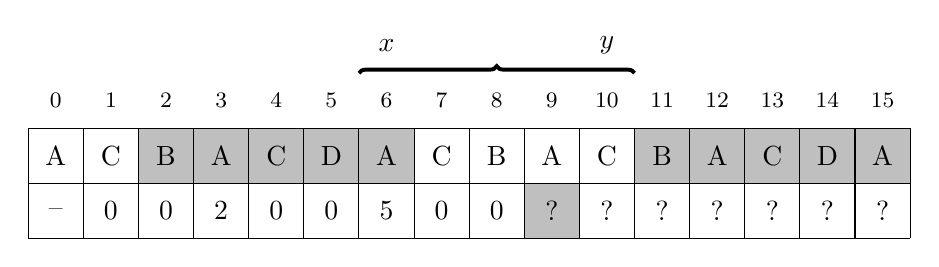
\begin{tikzpicture}[scale=0.7]
\fill[color=lightgray] (9,0) rectangle (10,1);
\fill[color=lightgray] (2,1) rectangle (7,2);
\fill[color=lightgray] (11,1) rectangle (16,2);


\draw (0,0) grid (16,2);

\node at (0.5, 1.5) {A};
\node at (1.5, 1.5) {C};
\node at (2.5, 1.5) {B};
\node at (3.5, 1.5) {A};
\node at (4.5, 1.5) {C};
\node at (5.5, 1.5) {D};
\node at (6.5, 1.5) {A};
\node at (7.5, 1.5) {C};
\node at (8.5, 1.5) {B};
\node at (9.5, 1.5) {A};
\node at (10.5, 1.5) {C};
\node at (11.5, 1.5) {B};
\node at (12.5, 1.5) {A};
\node at (13.5, 1.5) {C};
\node at (14.5, 1.5) {D};
\node at (15.5, 1.5) {A};

\node at (0.5, 0.5) {--};
\node at (1.5, 0.5) {0};
\node at (2.5, 0.5) {0};
\node at (3.5, 0.5) {2};
\node at (4.5, 0.5) {0};
\node at (5.5, 0.5) {0};
\node at (6.5, 0.5) {5};
\node at (7.5, 0.5) {0};
\node at (8.5, 0.5) {0};
\node at (9.5, 0.5) {?};
\node at (10.5, 0.5) {?};
\node at (11.5, 0.5) {?};
\node at (12.5, 0.5) {?};
\node at (13.5, 0.5) {?};
\node at (14.5, 0.5) {?};
\node at (15.5, 0.5) {?};

\draw [decoration={brace}, decorate, line width=0.5mm] (6,3.00) -- (11,3.00);

\node at (6.5,3.50) {$x$};
\node at (10.5,3.50) {$y$};


\footnotesize
\node at (0.5, 2.5) {0};
\node at (1.5, 2.5) {1};
\node at (2.5, 2.5) {2};
\node at (3.5, 2.5) {3};
\node at (4.5, 2.5) {4};
\node at (5.5, 2.5) {5};
\node at (6.5, 2.5) {6};
\node at (7.5, 2.5) {7};
\node at (8.5, 2.5) {8};
\node at (9.5, 2.5) {9};
\node at (10.5, 2.5) {10};
\node at (11.5, 2.5) {11};
\node at (12.5, 2.5) {12};
\node at (13.5, 2.5) {13};
\node at (14.5, 2.5) {14};
\node at (15.5, 2.5) {15};

%\draw[thick,<->] (11.5,-0.25) .. controls (11,-1.25) and (3,-1.25) .. (2.5,-0.25);
\end{tikzpicture}
\end{center}


Resulta que $\texttt{z}[9]=7$, de manera que el nou rang $[x,y]$ és $[9,15]$:


\begin{center}
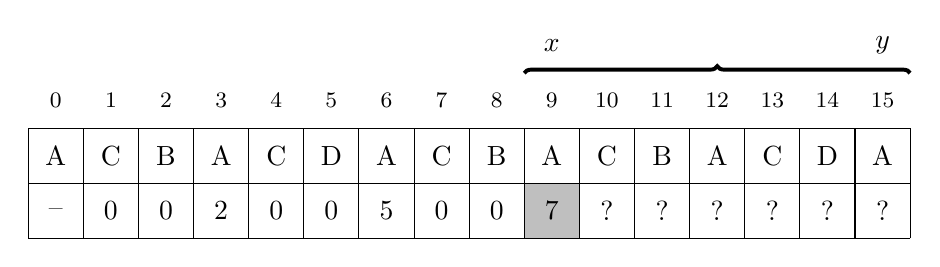
\begin{tikzpicture}[scale=0.7]
\fill[color=lightgray] (9,0) rectangle (10,1);
\draw (0,0) grid (16,2);

\node at (0.5, 1.5) {A};
\node at (1.5, 1.5) {C};
\node at (2.5, 1.5) {B};
\node at (3.5, 1.5) {A};
\node at (4.5, 1.5) {C};
\node at (5.5, 1.5) {D};
\node at (6.5, 1.5) {A};
\node at (7.5, 1.5) {C};
\node at (8.5, 1.5) {B};
\node at (9.5, 1.5) {A};
\node at (10.5, 1.5) {C};
\node at (11.5, 1.5) {B};
\node at (12.5, 1.5) {A};
\node at (13.5, 1.5) {C};
\node at (14.5, 1.5) {D};
\node at (15.5, 1.5) {A};

\node at (0.5, 0.5) {--};
\node at (1.5, 0.5) {0};
\node at (2.5, 0.5) {0};
\node at (3.5, 0.5) {2};
\node at (4.5, 0.5) {0};
\node at (5.5, 0.5) {0};
\node at (6.5, 0.5) {5};
\node at (7.5, 0.5) {0};
\node at (8.5, 0.5) {0};
\node at (9.5, 0.5) {7};
\node at (10.5, 0.5) {?};
\node at (11.5, 0.5) {?};
\node at (12.5, 0.5) {?};
\node at (13.5, 0.5) {?};
\node at (14.5, 0.5) {?};
\node at (15.5, 0.5) {?};

\draw [decoration={brace}, decorate, line width=0.5mm] (9,3.00) -- (16,3.00);

\node at (9.5,3.50) {$x$};
\node at (15.5,3.50) {$y$};


\footnotesize
\node at (0.5, 2.5) {0};
\node at (1.5, 2.5) {1};
\node at (2.5, 2.5) {2};
\node at (3.5, 2.5) {3};
\node at (4.5, 2.5) {4};
\node at (5.5, 2.5) {5};
\node at (6.5, 2.5) {6};
\node at (7.5, 2.5) {7};
\node at (8.5, 2.5) {8};
\node at (9.5, 2.5) {9};
\node at (10.5, 2.5) {10};
\node at (11.5, 2.5) {11};
\node at (12.5, 2.5) {12};
\node at (13.5, 2.5) {13};
\node at (14.5, 2.5) {14};
\node at (15.5, 2.5) {15};

% \draw[thick,<->] (9.5,-0.25) .. controls (9,-1.25) and (4,-1.25) .. (3.5,-0.25);
\end{tikzpicture}
\end{center}


Després d'això, es poden determinar tots els valors restants del
Z-vector fent servir la informació ja emmagatzemada al Z-vector:


\begin{center}
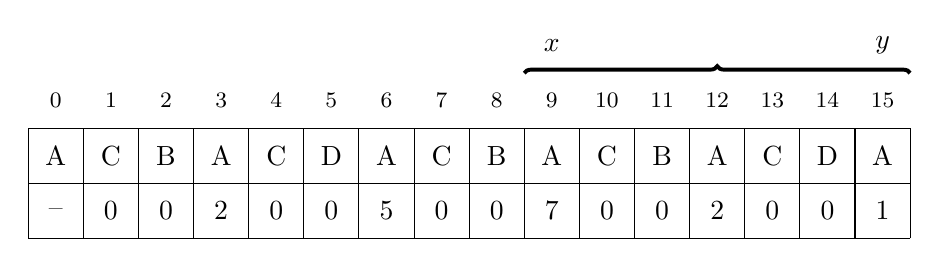
\begin{tikzpicture}[scale=0.7]
\draw (0,0) grid (16,2);

\node at (0.5, 1.5) {A};
\node at (1.5, 1.5) {C};
\node at (2.5, 1.5) {B};
\node at (3.5, 1.5) {A};
\node at (4.5, 1.5) {C};
\node at (5.5, 1.5) {D};
\node at (6.5, 1.5) {A};
\node at (7.5, 1.5) {C};
\node at (8.5, 1.5) {B};
\node at (9.5, 1.5) {A};
\node at (10.5, 1.5) {C};
\node at (11.5, 1.5) {B};
\node at (12.5, 1.5) {A};
\node at (13.5, 1.5) {C};
\node at (14.5, 1.5) {D};
\node at (15.5, 1.5) {A};

\node at (0.5, 0.5) {--};
\node at (1.5, 0.5) {0};
\node at (2.5, 0.5) {0};
\node at (3.5, 0.5) {2};
\node at (4.5, 0.5) {0};
\node at (5.5, 0.5) {0};
\node at (6.5, 0.5) {5};
\node at (7.5, 0.5) {0};
\node at (8.5, 0.5) {0};
\node at (9.5, 0.5) {7};
\node at (10.5, 0.5) {0};
\node at (11.5, 0.5) {0};
\node at (12.5, 0.5) {2};
\node at (13.5, 0.5) {0};
\node at (14.5, 0.5) {0};
\node at (15.5, 0.5) {1};

\draw [decoration={brace}, decorate, line width=0.5mm] (9,3.00) -- (16,3.00);

\node at (9.5,3.50) {$x$};
\node at (15.5,3.50) {$y$};


\footnotesize
\node at (0.5, 2.5) {0};
\node at (1.5, 2.5) {1};
\node at (2.5, 2.5) {2};
\node at (3.5, 2.5) {3};
\node at (4.5, 2.5) {4};
\node at (5.5, 2.5) {5};
\node at (6.5, 2.5) {6};
\node at (7.5, 2.5) {7};
\node at (8.5, 2.5) {8};
\node at (9.5, 2.5) {9};
\node at (10.5, 2.5) {10};
\node at (11.5, 2.5) {11};
\node at (12.5, 2.5) {12};
\node at (13.5, 2.5) {13};
\node at (14.5, 2.5) {14};
\node at (15.5, 2.5) {15};

\end{tikzpicture}
\end{center}


\subsubsection{Ús del Z-vector}

Sovint és qüestió de gustos si s'ha d'utilitzar string hashing o
l'algorisme Z. A diferència del hashing, l'algoritsme Z sempre
funciona i no hi ha cap risc de col·lisions. D'altra banda,
l'algorisme Z és més difícil d'implementar i alguns problemes només es
poden resoldre mitjançant hashing.

Com a exemple, considerem de nou el problema de cerca de patrons, on
la nostra tasca és trobar les ocurrències d'un patró $p$ en una cadena
$s$. Ja hem resolt aquest problema de manera eficient utilitzant el
hashing de cadena, però l'algorisme Z proporciona una altra manera de
resoldre el problema.

Una idea habitual en el processament de cadenes és construir una
cadena que consta de múltiples cadenes separades per caràcters
especials. En aquest problema, podem construir una cadena
$p$\texttt{\#}$s$, on $p$ i $s$ estan separats per un caràcter
especial \texttt{\#} que no apareix a les cadenes. El Z-vector de
$p$\texttt{\#}$s$ ens indica les posicions on $p$ apareix a $s$,
perquè aquestes posicions contenen la longitud de $p$.

Per exemple, si $s=$\texttt{HATTIVATTI} i $p=$\texttt{ATT}, el
Z-vector és els següent:


\begin{center}
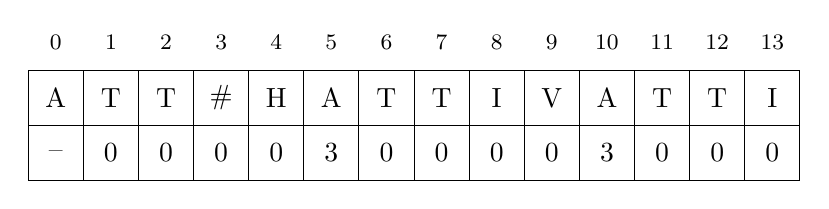
\begin{tikzpicture}[scale=0.7]
\draw (0,0) grid (14,2);

\node at (0.5, 1.5) {A};
\node at (1.5, 1.5) {T};
\node at (2.5, 1.5) {T};
\node at (3.5, 1.5) {\#};
\node at (4.5, 1.5) {H};
\node at (5.5, 1.5) {A};
\node at (6.5, 1.5) {T};
\node at (7.5, 1.5) {T};
\node at (8.5, 1.5) {I};
\node at (9.5, 1.5) {V};
\node at (10.5, 1.5) {A};
\node at (11.5, 1.5) {T};
\node at (12.5, 1.5) {T};
\node at (13.5, 1.5) {I};

\node at (0.5, 0.5) {--};
\node at (1.5, 0.5) {0};
\node at (2.5, 0.5) {0};
\node at (3.5, 0.5) {0};
\node at (4.5, 0.5) {0};
\node at (5.5, 0.5) {3};
\node at (6.5, 0.5) {0};
\node at (7.5, 0.5) {0};
\node at (8.5, 0.5) {0};
\node at (9.5, 0.5) {0};
\node at (10.5, 0.5) {3};
\node at (11.5, 0.5) {0};
\node at (12.5, 0.5) {0};
\node at (13.5, 0.5) {0};

\footnotesize
\node at (0.5, 2.5) {0};
\node at (1.5, 2.5) {1};
\node at (2.5, 2.5) {2};
\node at (3.5, 2.5) {3};
\node at (4.5, 2.5) {4};
\node at (5.5, 2.5) {5};
\node at (6.5, 2.5) {6};
\node at (7.5, 2.5) {7};
\node at (8.5, 2.5) {8};
\node at (9.5, 2.5) {9};
\node at (10.5, 2.5) {10};
\node at (11.5, 2.5) {11};
\node at (12.5, 2.5) {12};
\node at (13.5, 2.5) {13};
\end{tikzpicture}
\end{center}


Les posicions 5 i 10 contenen el valor 3, la qual cosa significa que
el patró \texttt{ATT} apareix a les posicions corresponents de
\texttt{HATTIVATTI}.

La complexitat temporal de l'algorisme resultant és lineal, perquè
n'hi ha prou per construir el Z-vector i repassar els seus valors.

\subsubsection{Implementació}

Aquí hi ha una breu implementació de l'algorisme Z que retorna el Z-vector.


\begin{lstlisting}
vector<int> z(string s) {
    int n = s.size();
    vector<int> z(n);
    int x = 0, y = 0;
    for (int i = 1; i < n; i++) {
        z[i] = max(0,min(z[i-x],y-i+1));
        while (i+z[i] < n && s[z[i]] == s[i+z[i]]) {
            x = i; y = i+z[i]; z[i]++;
        }
    }
    return z;
}
\end{lstlisting}

